\chapter{Introduction}
\label{cp:introduction}
One of the least obstructive and most feasible methods of measuring airspeed or flow velocity is by measuring the dynamic pressure of the flow. The dynamic pressure of a flow is related to the velocity via \autoref{eq:dynamic_pressure}.

\begin{equation} \label{eq:dynamic_pressure}
    q = \frac{1}{2} \rho V^2
\end{equation}

\noindent{}where \gls{q} is the dynamic pressure, \gls{rho} is the density, and \gls{V} is the velocity \citep{lab2-manual}.

Since the dynamic pressure, \gls{q}, is related to the total and static pressure (see \autoref{cp:methodology}), a pitot tube—which simultaneously measures total and static pressure—is commonly used to calculate \gls{q}.

\begin{figure}[htpb]
    \centering
    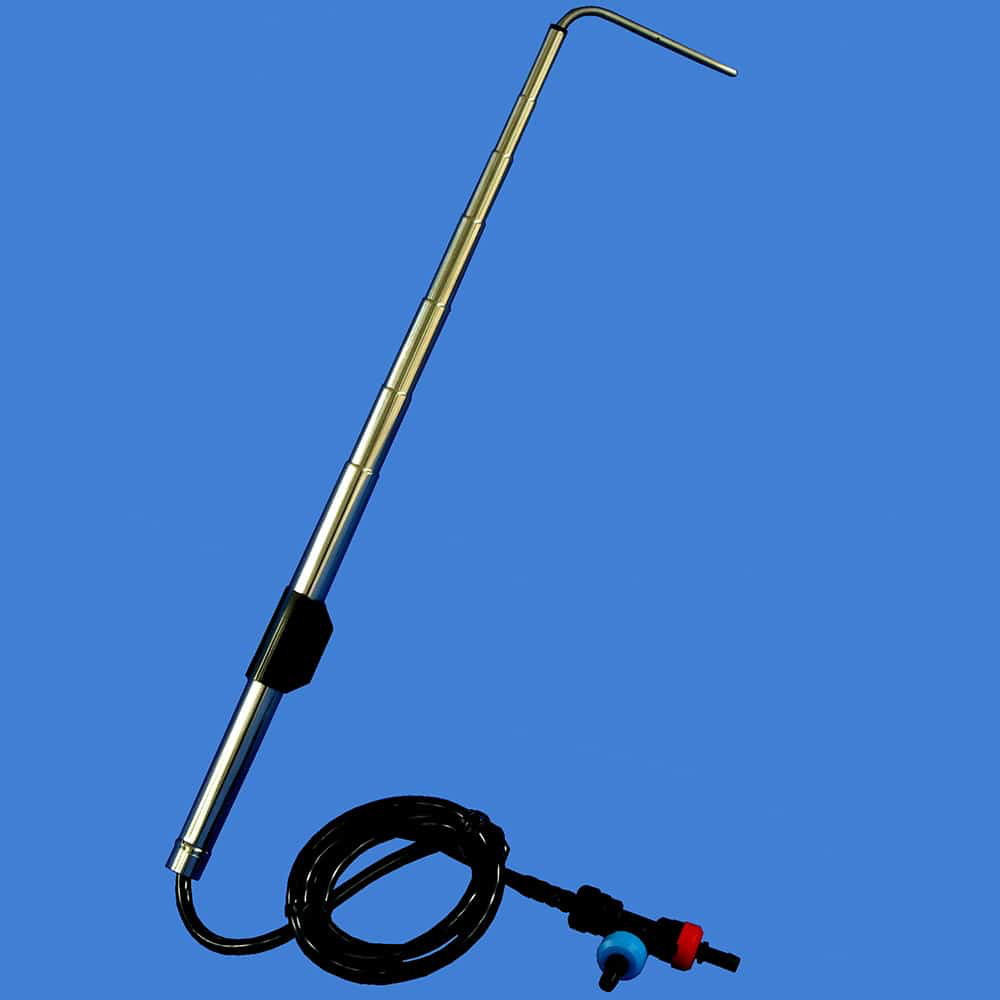
\includegraphics[width=0.5\linewidth]{Figures/pitot_tube.png}
    \caption[Photo of a pitot tube]{A photograph of a pitot tube available for purchase on \url{https://www.ttseries.com}.}
\end{figure}

For some aerodynamic tests, pitot tubes may be impractical or may obstruct the flow in a significant way. In these situations, an alternative method must be used to measure the airspeed in the test chamber. One solution is to take static pressure measurements at two points upstream of the test chamber and use a constant coefficient to relate the static pressure differential to the dynamic pressure in the test chamber.

In the low-speed wind tunnel, the two static pressure ports are located at point A and point E as shown in \autoref{fig:lab_drawing}:

\begin{figure}[htpb]
    \centering
    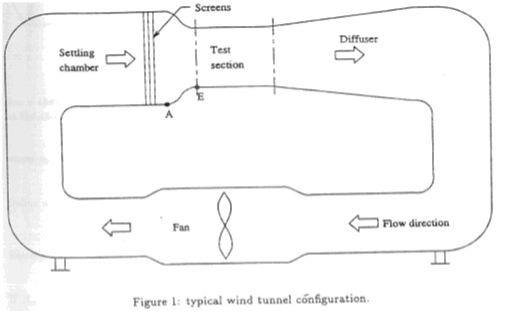
\includegraphics[width=\linewidth]{Figures/wind_tunnel_drawing.png}
    \caption[Drawing of the undergraduate wind tunnel configuration]{A drawing of the undergraduate wind tunnel, denoting the flow of air and points A and E \citep{lab2-manual}.}
    \label{fig:lab_drawing}
\end{figure}
 
Once we have calibrated the wind tunnel by following the procedure outlined in \autoref{cp:methodology} and determined the calibration constant, \gls{K}, only the static pressure differential measured from points A and E will be required to estimate the velocity in the test chamber.
